\documentclass[conference]{IEEEtran}

\usepackage[utf8]{inputenc}
\usepackage[T1]{fontenc}
\usepackage{amsmath,amssymb,amsfonts}
\usepackage{graphicx}
\usepackage[caption=false,font=footnotesize]{subfig}
\usepackage{booktabs}
\usepackage{hyperref}
\usepackage{array}
\usepackage{multirow}
\usepackage{url}
\usepackage{microtype}
\usepackage{float}

\graphicspath{{figures/}}

\title{Graph Cut Image Segmentation Pipeline for Foreground--Background Separation}

\author{
  \IEEEauthorblockN{Madhav Kataria}
  \IEEEauthorblockA{
    Roll No: B23CH1025 \\
    Computer Vision Assignment 2
  }
}

\begin{document}

\maketitle

\begin{abstract}
This report presents a complete image segmentation pipeline based on graph cut optimization for foreground--background separation under sparse user guidance. The implementation models foreground and background appearance with histogram-based unary terms in Lab color space, enforces spatial coherence through contrast-sensitive pairwise smoothness costs, and solves the resulting binary labeling problem using min-cut / max-flow. The pipeline further performs iterative model refinement, artifact mitigation, and final overlay generation for visually coherent outputs. Experiments on three bundled benchmark images (\textit{astronaut}, \textit{coffee}, and \textit{chelsea}) show that graph cut substantially reduces energy, suppresses fragmentation relative to a unary-only baseline, and yields clean, submission-ready segmentation outputs without relying on ground-truth masks.
\end{abstract}

\begin{IEEEkeywords}
graph cut, image segmentation, min-cut / max-flow, unary cost, pairwise smoothness, interactive segmentation
\end{IEEEkeywords}

\section{Problem Statement}
The goal of this assignment is to construct a full foreground--background segmentation pipeline using graph cut rather than a high-level automated API. The required system must:
\begin{itemize}
  \item represent an image as a graph with one node per pixel,
  \item define unary (data) and pairwise (smoothness) costs,
  \item solve the labeling problem with min-cut / max-flow,
  \item explain the roles of the source and sink terminals,
  \item model foreground and background appearance from user annotations,
  \item iteratively refine the segmentation,
  \item mitigate artifacts such as isolated regions and jagged edges,
  \item produce a clean final mask and overlay, and
  \item compare naive unary-only segmentation against graph-cut segmentation.
\end{itemize}

To satisfy these requirements, the repository bundles three deterministic images and corresponding sparse foreground/background scribble annotations. Bounding boxes are also supported as weak initialization constraints, but the primary experiments use scribbles because they map directly to hard source/sink seed constraints.

\section{Methodology}

\subsection{Graph Construction}
Each image is modeled as an undirected graph \(G = (V, E)\), where each pixel \(p \in V\) is connected to two terminals: the \textbf{source} \(S\), representing the foreground label, and the \textbf{sink} \(T\), representing the background label. In addition, each pixel is connected to its 8-neighborhood in order to promote local label consistency while respecting image boundaries.

\subsection{Energy Formulation}
The segmentation is obtained by minimizing the binary energy
\begin{equation}
E(L) = E_{\text{data}}(L) + \lambda E_{\text{smooth}}(L),
\end{equation}
where \(L_p \in \{\text{FG}, \text{BG}\}\) is the label of pixel \(p\), \(E_{\text{data}}\) is the unary data term, and \(E_{\text{smooth}}\) is the pairwise regularization term. The smoothness coefficient \(\lambda\) controls the trade-off between appearance fidelity and boundary regularity.

The data term is defined as
\begin{equation}
E_{\text{data}}(L) = \sum_p D_p(L_p),
\end{equation}
where \(D_p(\text{FG})\) and \(D_p(\text{BG})\) are negative log-likelihood costs derived from the foreground and background appearance models.

The pairwise term is defined over the neighborhood system \(\mathcal{N}\):
\begin{equation}
E_{\text{smooth}}(L) = \sum_{(p,q)\in\mathcal{N}} w_{pq}[L_p \neq L_q].
\end{equation}
Here, \(w_{pq}\) is a contrast-sensitive weight:
\begin{equation}
w_{pq} = \frac{1}{\operatorname{dist}(p,q)} \exp\left(-\beta \lVert I_p - I_q \rVert^2\right),
\end{equation}
with \(\beta\) estimated from the average squared color difference between neighboring pixels. This formulation penalizes label discontinuities strongly in smooth regions, but allows cuts to align with strong intensity or color edges.

\subsection{Unary Costs and Source / Sink Roles}
Unary costs are encoded as terminal capacities. For each pixel \(p\),
\begin{itemize}
  \item the edge from \(S\) to \(p\) receives the cost of assigning \(p\) to the background,
  \item the edge from \(p\) to \(T\) receives the cost of assigning \(p\) to the foreground.
\end{itemize}
As a result, the minimum cut partitions pixels into the source-connected foreground set and the sink-connected background set while minimizing the total energy.

Foreground and background scribbles are treated as hard constraints by assigning a prohibitive cost to inconsistent labels. This ensures that user-provided seeds always remain on the correct side of the cut.
In addition, the implementation augments the histogram-based unary term with a weak distance-to-seed prior and an optional outside-box penalty. These soft spatial cues discourage implausible foreground leakage while preserving the graph-cut formulation required by the assignment.

\subsection{Foreground--Background Modeling}
Foreground and background appearance are modeled with histogram-based color likelihoods in Lab space. Let \(\mathcal{F}\) and \(\mathcal{B}\) denote the sets of foreground and background seed pixels. Separate 3D histograms are estimated over the quantized Lab channels, Laplace-smoothed to avoid zero-probability bins, and normalized to produce class-conditional likelihoods:
\begin{equation}
P(I_p \mid \text{FG}), \qquad P(I_p \mid \text{BG}).
\end{equation}
Unary costs are then computed as
\begin{equation}
D_p(\text{FG}) = -\log P(I_p \mid \text{FG}), \qquad D_p(\text{BG}) = -\log P(I_p \mid \text{BG}).
\end{equation}

\subsection{Iterative Optimization}
The initial appearance models are estimated from the user scribbles. Graph cut is then solved, and the resulting mask is used to re-estimate the appearance models while preserving the original seeds. This process is repeated for a small number of iterations or until the mask change ratio falls below a convergence threshold. Recording energy per iteration makes the refinement dynamics explicit.

\subsection{Artifact Mitigation and Final Output}
The raw graph-cut mask is post-processed through:
\begin{itemize}
  \item removal of small isolated connected components,
  \item elimination of small holes,
  \item morphological opening/closing, and
  \item Gaussian smoothing followed by seed-preserving connected-component selection.
\end{itemize}
The refined mask is finally overlaid on the original image to produce an interpretable final segmentation result.

\subsection{Naive Baseline}
For comparison, a naive segmentation baseline is included. It uses the \emph{same} unary cost model and the same user annotations, but omits pairwise smoothness and graph optimization. Each pixel is classified independently according to the lower unary cost. This provides a fair baseline that isolates the value of graph-based regularization.

\section{Implementation Details}

\subsection{Repository Organization}
The project is structured as follows:
\begin{itemize}
  \item \texttt{src/}: graph cut pipeline, data I/O, modeling, optimization, evaluation, visualization, and report asset generation.
  \item \texttt{tests/}: unit tests and an end-to-end smoke test.
  \item \texttt{configs/}: dataset and experiment YAML configurations.
  \item \texttt{data/}: bundled images and scribble annotations.
  \item \texttt{results/}: generated masks, overlays, comparison panels, and summary metrics.
  \item \texttt{report/}: LaTeX report source and synchronized figures.
\end{itemize}

\subsection{Main Components}
The core implementation is divided across the following modules:
\begin{itemize}
  \item \texttt{data\_io.py}: image loading, resizing, annotation parsing, and output serialization.
  \item \texttt{modeling.py}: Lab conversion, histogram estimation, and unary cost computation.
  \item \texttt{graph\_construction.py}: contrast-sensitive pairwise weights and graph assembly.
  \item \texttt{maxflow\_solver.py}: min-cut / max-flow execution using \texttt{PyMaxflow}.
  \item \texttt{optimization.py}: iterative graph-cut refinement loop.
  \item \texttt{refinement.py}: artifact mitigation for final mask cleanup.
  \item \texttt{evaluation.py}: energy computation and proxy quality metrics.
  \item \texttt{visualization.py}: overlay, comparison panel, and boundary visualization generation.
  \item \texttt{cli.py}: reproducible \texttt{prepare-data}, \texttt{run}, \texttt{evaluate}, and \texttt{all} commands.
\end{itemize}

\subsection{Configuration}
The experiments use Python 3.11 and a YAML-based configuration system. Key parameters include:
\begin{itemize}
  \item longest-side resize limit: 384 px,
  \item histogram bins: \(16 \times 16 \times 16\),
  \item smoothness weight: \(\lambda = 28\),
  \item hard seed cost: \(10^6\),
  \item distance-prior weight: 1.0,
  \item weak outside-box foreground penalty: 4.0,
  \item refinement closing radius: 1,
  \item refinement Gaussian smoothing: \(\sigma = 0.4\),
  \item maximum graph-cut iterations: 3.
\end{itemize}

\begin{figure}[!t]
  \centering
  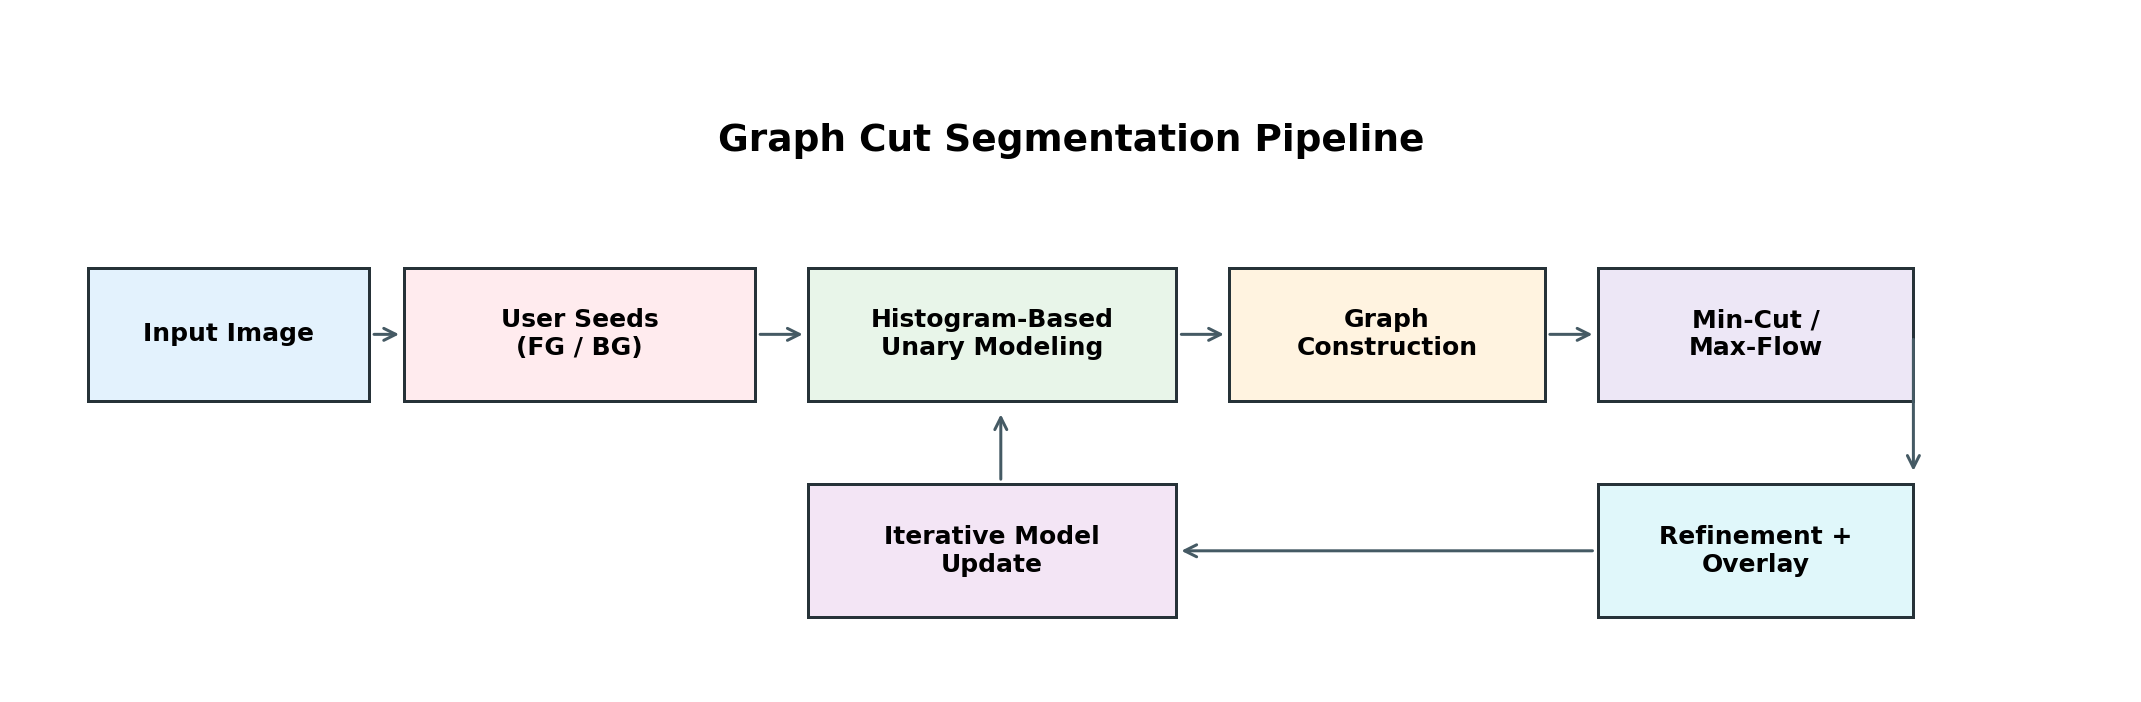
\includegraphics[width=\linewidth]{pipeline_overview.png}
  \caption{End-to-end segmentation workflow, including user guidance, unary modeling, graph cut, iterative refinement, and final overlay generation.}
  \label{fig:pipeline}
\end{figure}

\begin{figure}[!t]
  \centering
  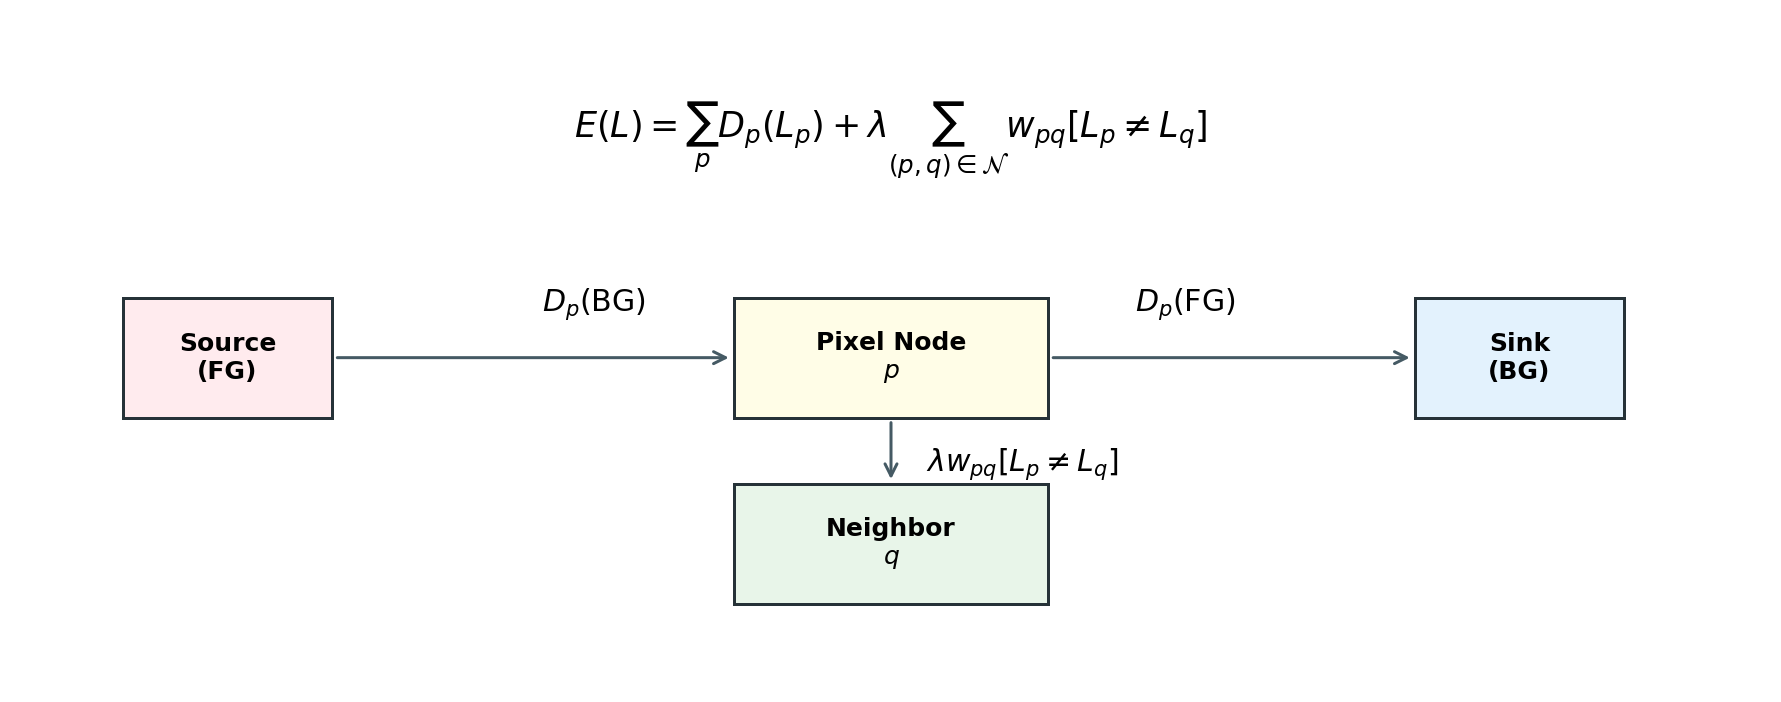
\includegraphics[width=\linewidth]{energy_graph_schematic.png}
  \caption{Graph construction and energy interpretation: the source models foreground, the sink models background, and pairwise neighborhood edges implement the smoothness term.}
  \label{fig:energy}
\end{figure}

\section{Results}

\subsection{Dataset}
\begin{table}[!t]
  \centering
  \caption{Bundled evaluation images and annotation setup}
  \begin{tabular}{>{\raggedright\arraybackslash}p{1.5cm} >{\raggedright\arraybackslash}p{2.0cm} >{\raggedright\arraybackslash}p{1.3cm} >{\raggedright\arraybackslash}p{1.6cm}}
    \toprule
    Image & Target & Resolution & Annotation \\
    \midrule
    astronaut & astronaut subject & \(512 \times 512\) & sparse FG/BG scribbles + weak box \\
    coffee & coffee cup & \(400 \times 600\) & sparse FG/BG scribbles + weak box \\
    chelsea & cat & \(300 \times 451\) & sparse FG/BG scribbles + weak box \\
    \bottomrule
  \end{tabular}
  \label{tab:dataset}
\end{table}

\subsection{Quantitative Comparison}
\begin{table*}[!t]
  \centering
  \caption{Naive vs graph-cut performance without ground-truth masks}
  \scriptsize
  \begin{tabular}{lrrrrrrrrrr}
    \toprule
    Image & Naive Energy & Graph-Cut Energy & Refined Energy & Naive Components & Refined Components & Naive Boundary & Refined Boundary & Refined Compactness & Refined Edge Align. & Refined Leakage \\
    \midrule
    astronaut & 1307712.98 & 587651.75 & 591253.81 & 642 & 1 & 13340.97 & 1645.07 & 0.1950 & 4.1792 & 0.0061 \\
    coffee    & 678988.58  & 401058.24 & 401186.18 & 304 & 1 & 3961.01  & 629.24  & 0.4389 & 3.1325 & 0.0000 \\
    chelsea   & 758224.66  & 345832.03 & 347021.97 & 145 & 1 & 9205.03  & 1067.07 & 0.4014 & 2.5509 & 0.0062 \\
    \bottomrule
  \end{tabular}
  \label{tab:results}
\end{table*}

The quantitative results show a consistent improvement over the naive baseline. Averaged across all three images, the refined graph-cut masks reduce total energy by 51.2\%, boundary length by 87.4\%, and connected-component count by 99.7\%. At the same time, the mean edge-alignment score improves from 2.24 to 3.29, and the mean bounding-box leakage ratio drops from 0.061 to 0.004. These trends indicate that graph cut improves not only smoothness and connectivity, but also boundary plausibility and spatial containment. The coffee example is especially strong: the refined mask reaches zero measured leakage while preserving a compact, single-component object.

\subsection{Qualitative Comparison}
\begin{figure*}[!t]
  \centering
  \subfloat[Astronaut scene]{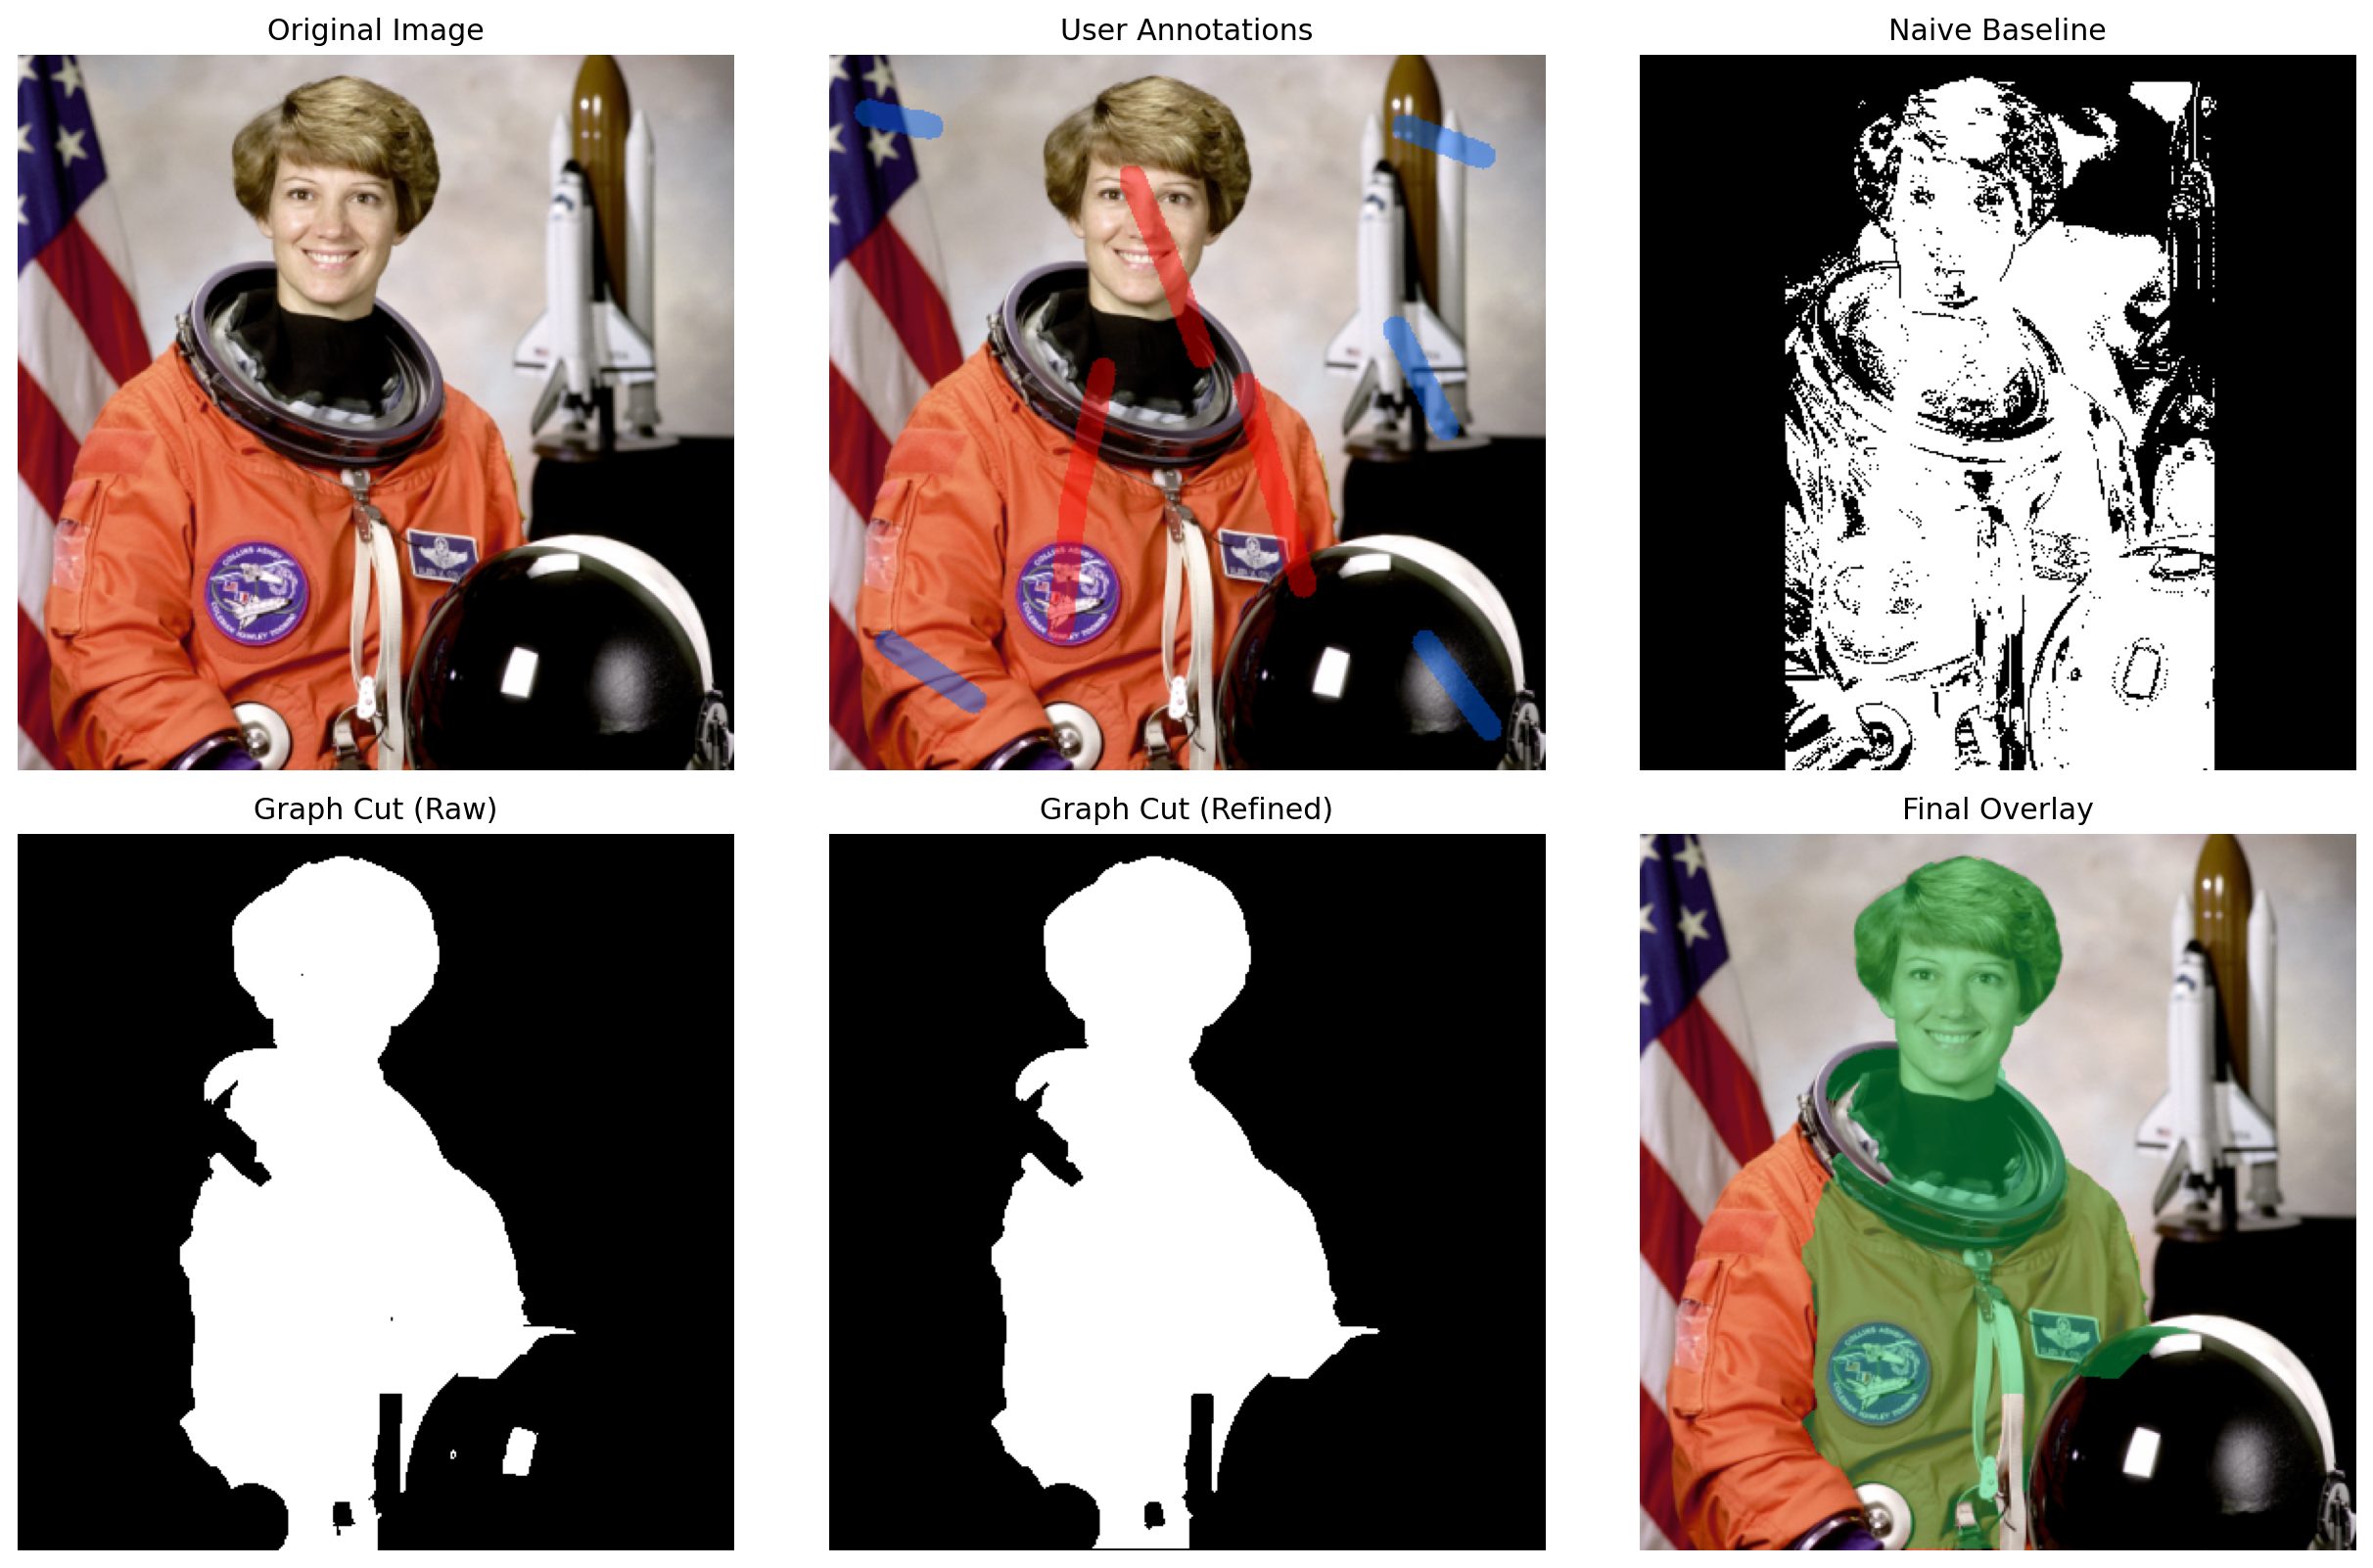
\includegraphics[width=0.32\linewidth]{astronaut_comparison.png}\label{fig:astronaut_cmp}}
  \hfill
  \subfloat[Coffee cup scene]{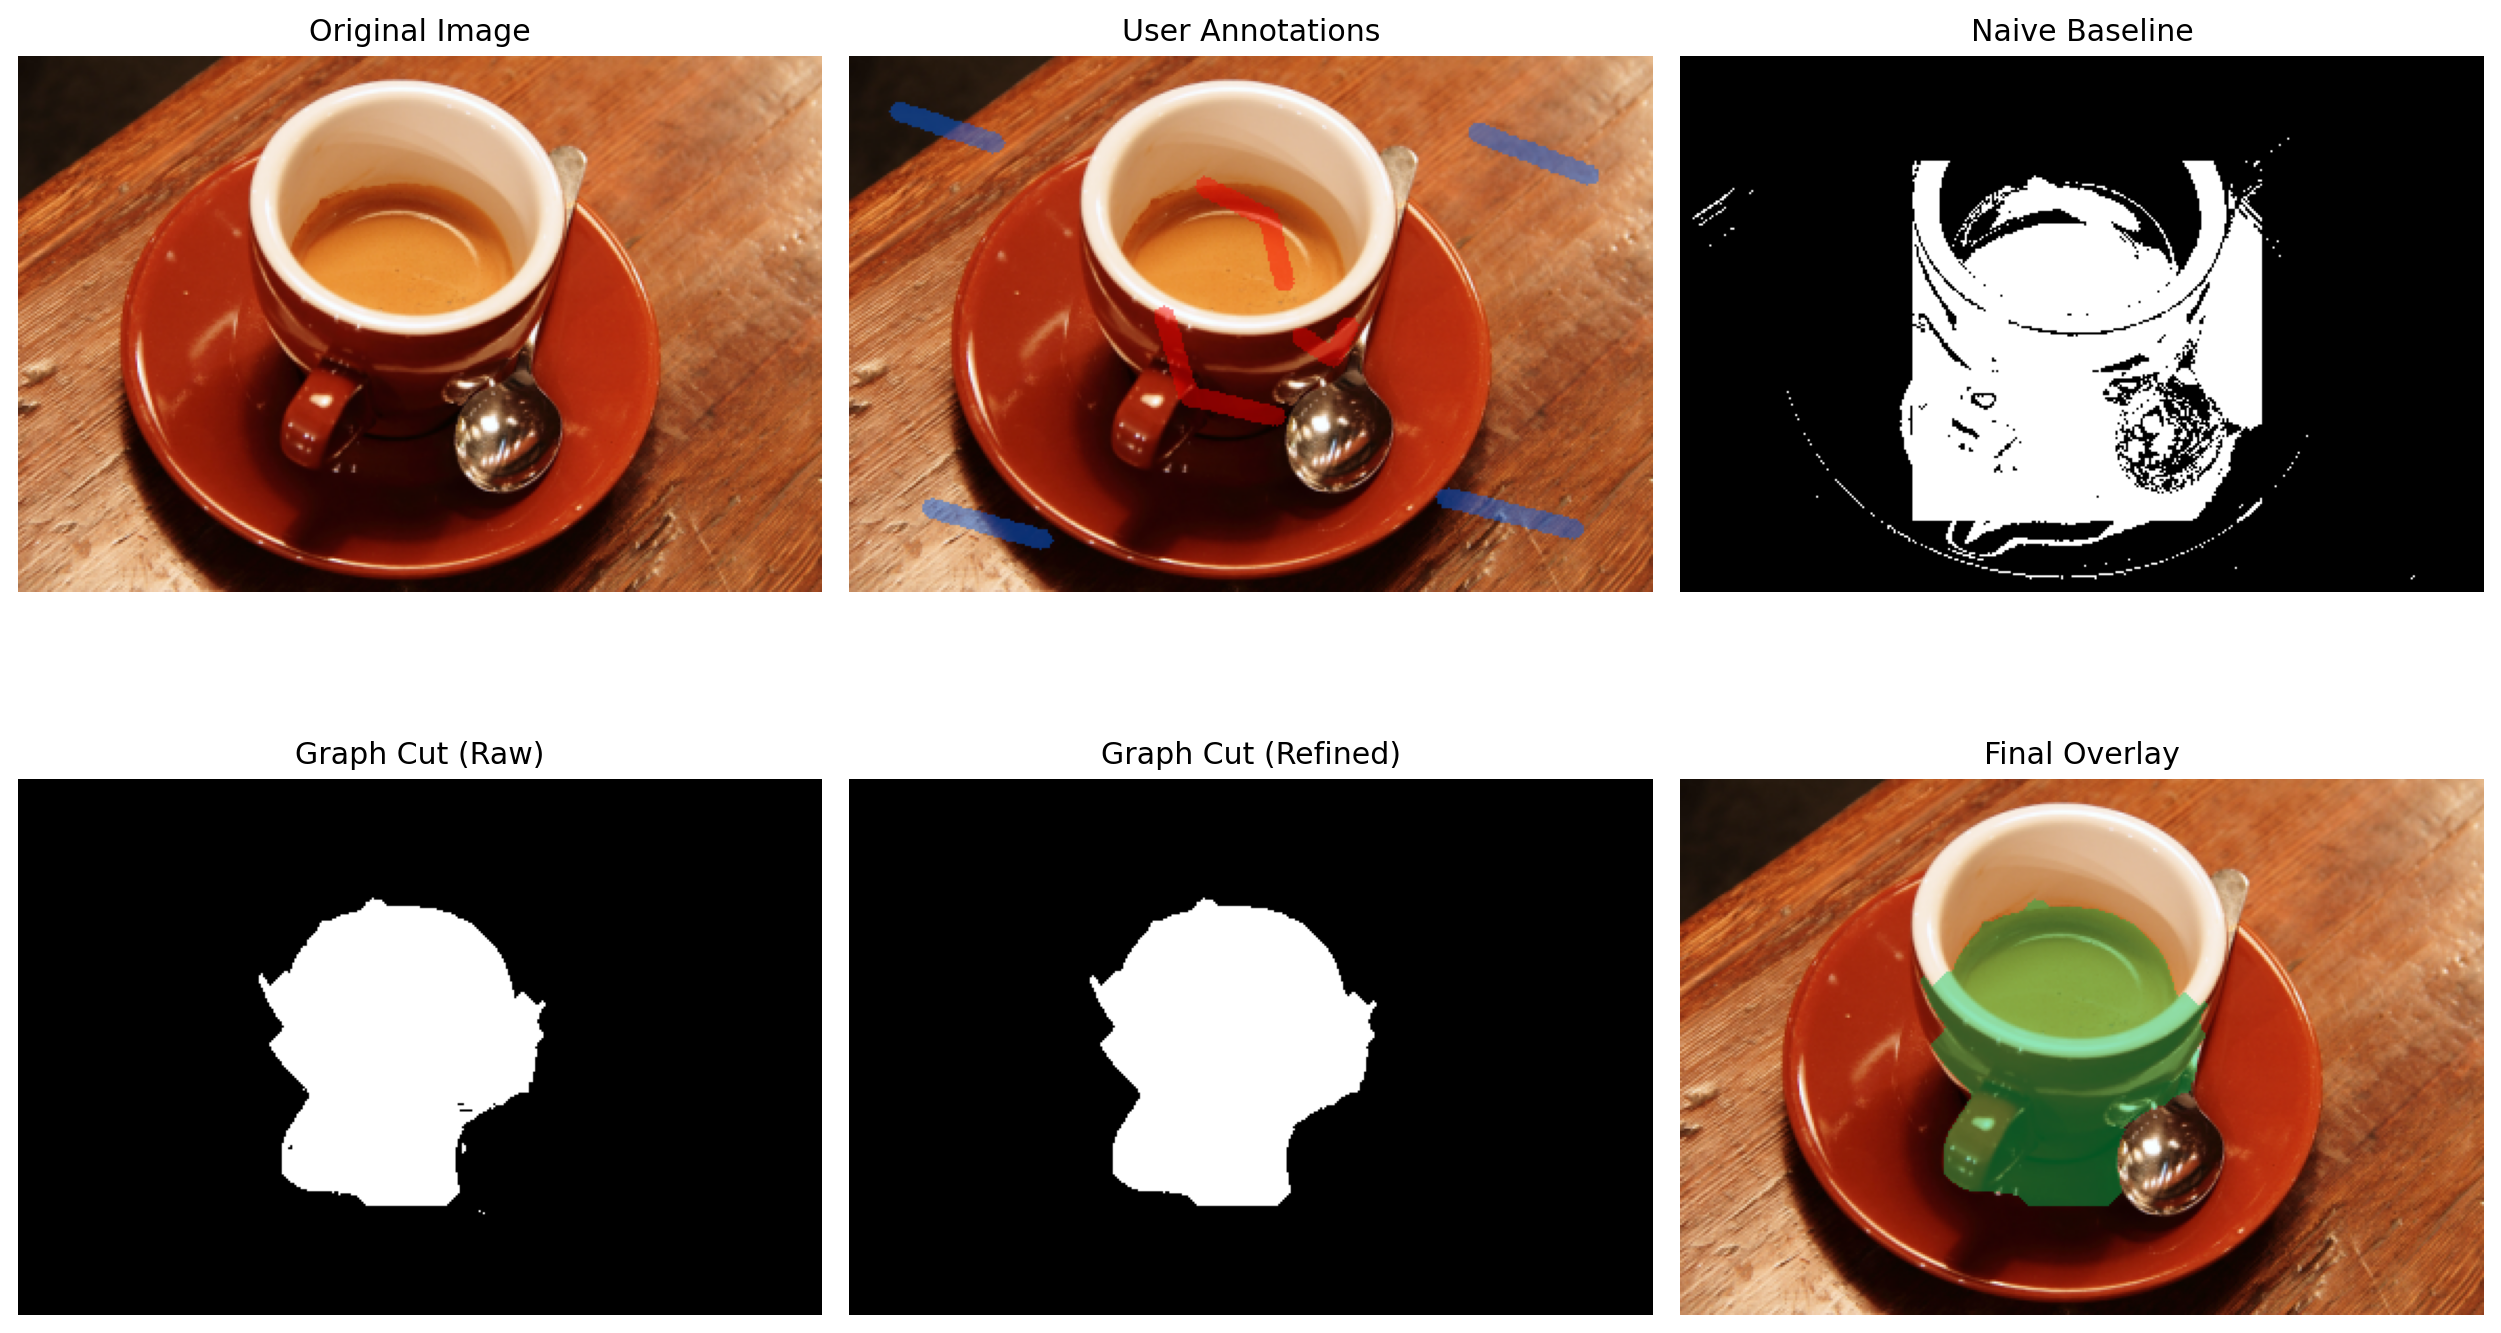
\includegraphics[width=0.32\linewidth]{coffee_comparison.png}\label{fig:coffee_cmp}}
  \hfill
  \subfloat[Cat scene]{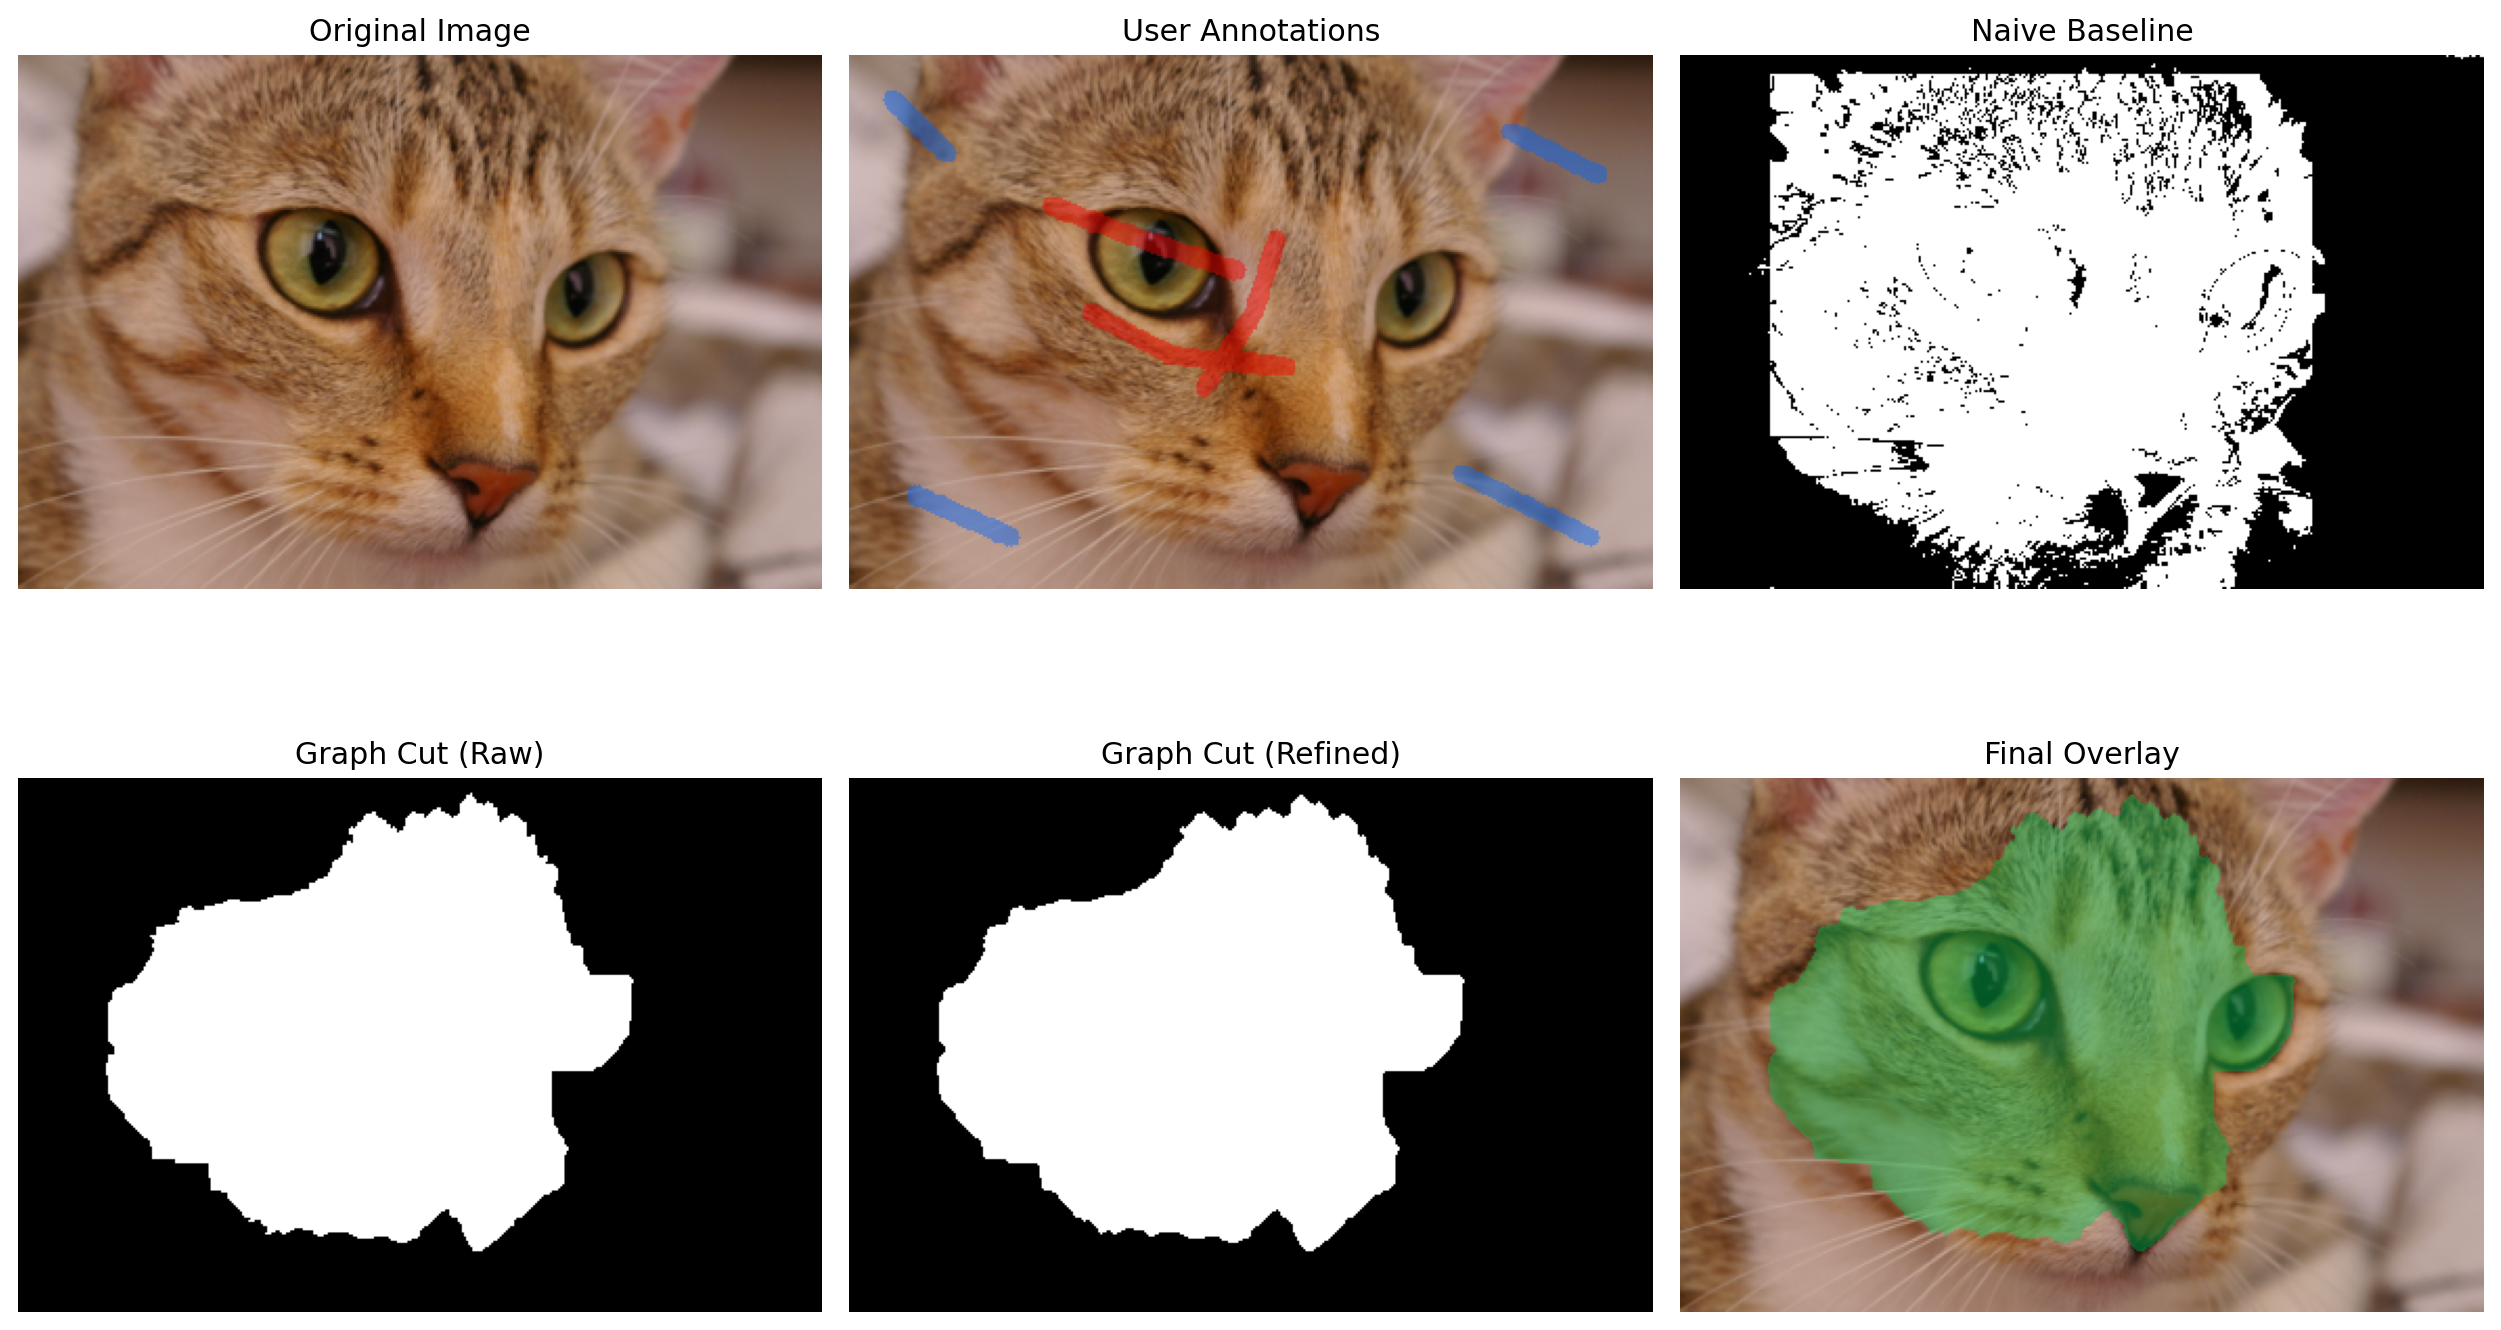
\includegraphics[width=0.32\linewidth]{chelsea_comparison.png}\label{fig:chelsea_cmp}}
  \caption{Per-image comparison panels showing the original image, user annotations, unary-only baseline, raw graph-cut output, refined graph-cut mask, and final overlay.}
  \label{fig:comparisons}
\end{figure*}

\begin{figure*}[!t]
  \centering
  \subfloat[Astronaut boundary refinement]{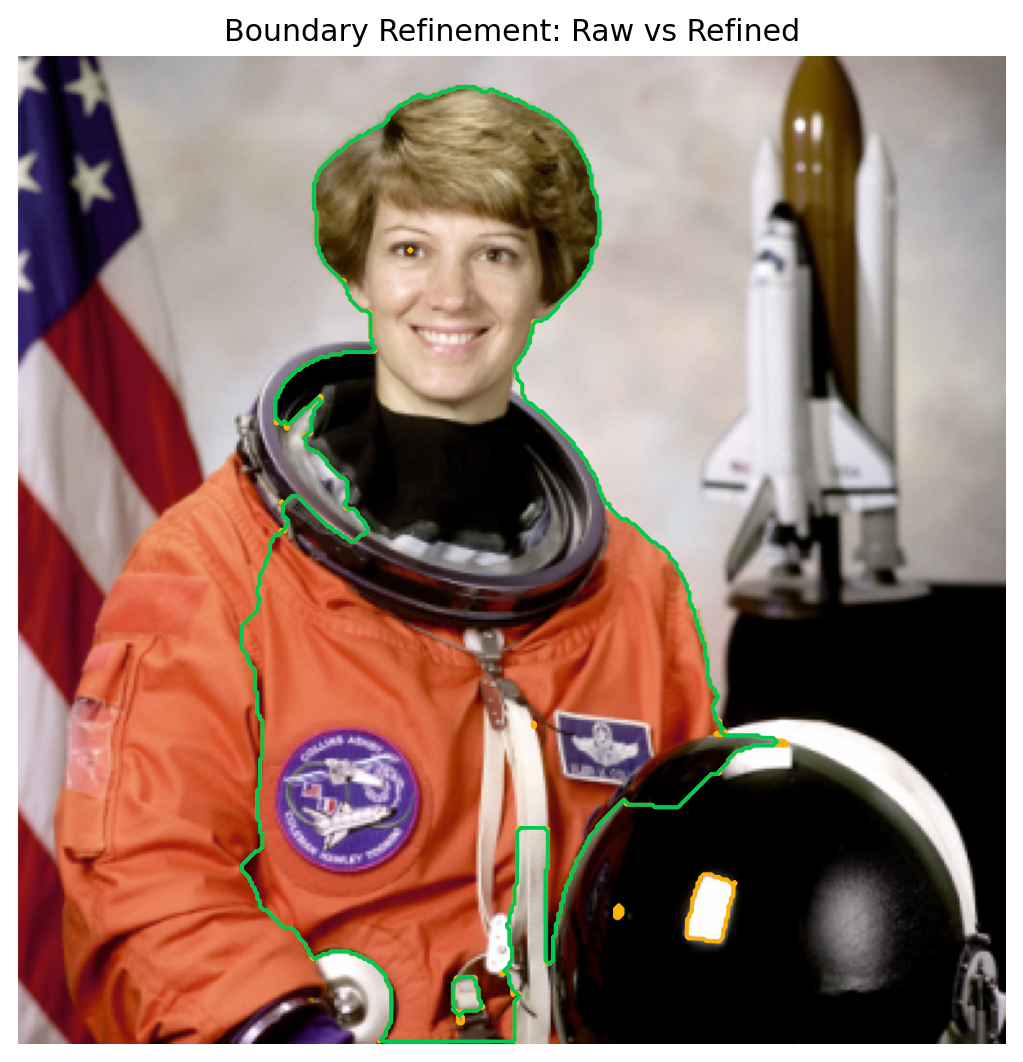
\includegraphics[width=0.32\linewidth]{astronaut_boundary.png}}
  \hfill
  \subfloat[Coffee boundary refinement]{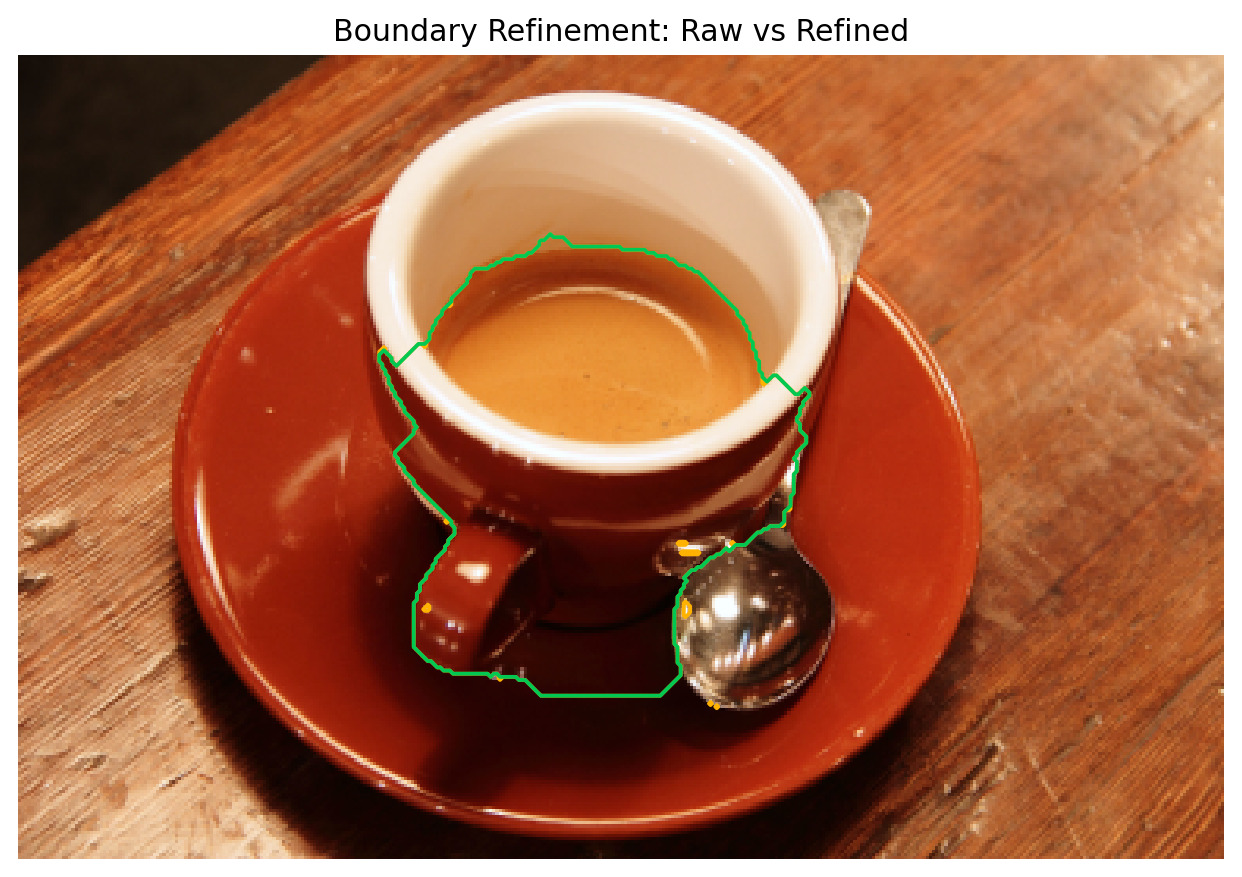
\includegraphics[width=0.32\linewidth]{coffee_boundary.png}}
  \hfill
  \subfloat[Cat boundary refinement]{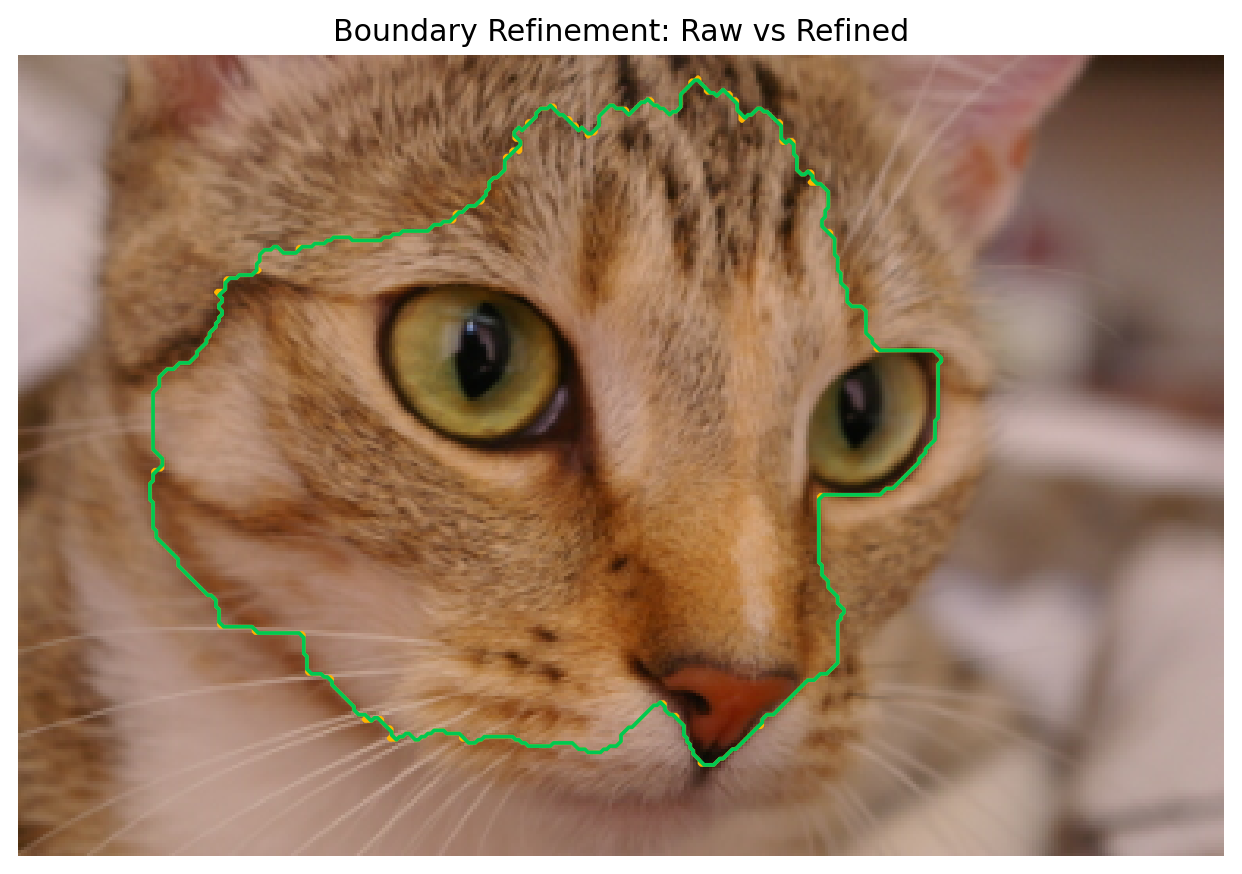
\includegraphics[width=0.32\linewidth]{chelsea_boundary.png}}
  \caption{Boundary refinement views highlighting the transition from raw graph-cut boundaries to the final refined segmentation.}
  \label{fig:boundaries}
\end{figure*}

\section{Deliverables}
This submission includes all deliverables requested in the assignment brief:
\begin{itemize}
  \item \textbf{Input Images.} At least three original images are used for segmentation: \textit{astronaut}, \textit{coffee}, and \textit{chelsea}. Their targets, resolutions, and annotation settings are listed in Table~\ref{tab:dataset}.
  \item \textbf{Codebase.} A well-structured and documented implementation is provided under \texttt{src/}, supported by tests under \texttt{tests/}, reproducible configuration files under \texttt{configs/}, bundled data under \texttt{data/}, and synchronized outputs under \texttt{results/}.
  \item \textbf{Results.} For each image, the submission provides segmentation masks and visualizations, including the annotation overlay, naive unary-only mask, raw graph-cut mask, refined graph-cut mask, boundary-refinement view, iteration-energy plot, and final overlay.
  \item \textbf{Report.} This document explains graph construction, unary and pairwise costs, the energy function, source/sink roles, foreground--background modeling, iterative optimization, artifact mitigation, and experimental observations.
  \item \textbf{Comparison.} A direct comparison between naive segmentation and graph-cut segmentation is provided quantitatively in Table~\ref{tab:results} and qualitatively in Fig.~\ref{fig:comparisons}.
\end{itemize}

\section{Analysis / Discussion}
Several observations emerge from the experiments:
\begin{itemize}
  \item \textbf{Graph cut vs naive classification.} The unary-only baseline is highly fragmented because it treats each pixel independently. Graph cut suppresses this behavior by coupling neighboring pixels through the smoothness term.
  \item \textbf{Benefit of iterative optimization.} Updating the appearance models after each cut stabilizes the mask and reduces energy over successive iterations. This is particularly useful when the initial scribbles only cover a small subset of the target object.
  \item \textbf{Effect of refinement.} The post-processing stage improves topological cleanliness by collapsing residual islands and smoothing boundaries. Although refined energy can rise slightly relative to the raw cut, the visual result is substantially more coherent and easier to interpret, with final masks reaching a single connected component in all three cases.
  \item \textbf{Stronger proxy evaluation.} Boundary length alone is not enough to judge segmentation quality. Adding edge alignment, compactness, and leakage metrics makes the evaluation more robust: the final masks are not only smoother, but also better aligned to image gradients and less likely to spill outside weak spatial support.
  \item \textbf{Image-specific behavior.} The coffee image is the cleanest case because the object has a strong geometric outline. The astronaut and cat cases are more challenging due to shared colors between foreground and background and fine texture around hair or fur.
\end{itemize}

Overall, the results are consistent with the theory behind graph cut segmentation: the data term captures class appearance, while the smoothness term injects the spatial regularity missing from naive classification.

\section{Limitations}
The current system remains binary and user-guided, so its quality depends on the placement and coverage of the provided scribbles. Histogram-based color modeling is lightweight and interpretable, but it can struggle when foreground and background share similar appearance statistics. The refinement stage improves mask quality, yet it is still a heuristic post-process rather than a learned boundary model. Finally, the quantitative evaluation uses proxy metrics because no ground-truth masks are provided.

\section{Conclusion}
This project delivers a complete graph-cut segmentation pipeline aligned with the assignment rubric. The implementation explicitly constructs the graph, defines unary and pairwise costs, solves min-cut / max-flow, models foreground/background appearance from user annotations, performs iterative refinement, mitigates artifacts, and produces final overlays. Both quantitative proxy metrics and qualitative comparison panels show that graph cut significantly outperforms a naive unary-only baseline in terms of energy, connected-component count, boundary regularity, edge alignment, and leakage control.

\appendices
\section{Execution Commands}
\begin{verbatim}
python -m src.cli prepare-data
python -m src.cli run --config configs/experiment.yaml
python -m src.cli evaluate --results-dir results
pytest
\end{verbatim}

\section{Project Structure}
\begin{verbatim}
src/      implementation modules
tests/    unit tests and smoke tests
configs/  experiment and dataset configuration
data/     bundled input images and annotations
results/  generated masks, overlays, plots, and summaries
report/   LaTeX source, bibliography, and synchronized figures
\end{verbatim}

\section{Key Output Files}
\begin{itemize}
  \item \texttt{results/case\_name/comparison\_panel.png}
  \item \texttt{results/case\_name/energy\_iterations.png}
  \item \texttt{results/case\_name/final\_overlay.png}
  \item \texttt{results/case\_name/metrics.json}
  \item \texttt{results/summary/metrics.csv}
  \item \texttt{results/summary/aggregate.json}
  \item \texttt{report/figures/*.png}
\end{itemize}

\bibliographystyle{IEEEtran}
\bibliography{references}

\end{document}
